\documentclass[conference]{IEEEtran}

\usepackage{amsmath}
\usepackage{graphicx}
\usepackage{subfigure}
\usepackage{color}
\usepackage{xspace}
\usepackage{url}

\newcommand{\lorem}               {\textcolor{green}{Lorem ipsum dolor sit amet, consectetur adipisicing elit, sed do eiusmod tempor incididunt ut labore et dolore magna aliqua. Ut enim ad minim veniam, quis nostrud exercitation ullamco laboris nisi ut aliquip ex ea commodo consequat. Duis aute irure dolor in reprehenderit in voluptate velit esse cillum dolore eu fugiat nulla pariatur. Excepteur sint occaecat cupidatat non proident, sunt in culpa qui officia deserunt mollit anim id est laborum.}}
%\newcommand{\thomas}[1]           {\textcolor{blue}{[Thomas] #1}}
\newcommand{\name}                {PEACH\xspace}
\newcommand{\smip}                {SmartMesh~IP\xspace}
\newcommand{\solmanager}          {{\tt solmanager}\xspace}
\newcommand{\solserver}           {{\tt solserver}\xspace}
\newcommand{\rpi}                 {Raspberry~Pi\xspace}

\graphicspath{{figs/}}

\begin{document}
\title{A Demo of the \name IoT-based Frost Event Prediction System for Precision Agriculture}

\author{
    \IEEEauthorblockN{
        Ivan~,
        Mario~,
        Marton~,
        Keoma~Brun-Laguna\IEEEauthorrefmark{1},
   }
   \IEEEauthorblockA{\IEEEauthorrefmark{1}~Inria-Paris, EVA Team, France}
}

\maketitle

\begin{abstract}
\end{abstract}

\begin{IEEEkeywords}
Smart Agriculture, Precision Agriculture, IoT.
\end{IEEEkeywords}

\IEEEpeerreviewmaketitle

%==============================================================================
\section{Overview}
\label{sec:overview}

% Reproducible Research

\begin{figure}
    \centering
    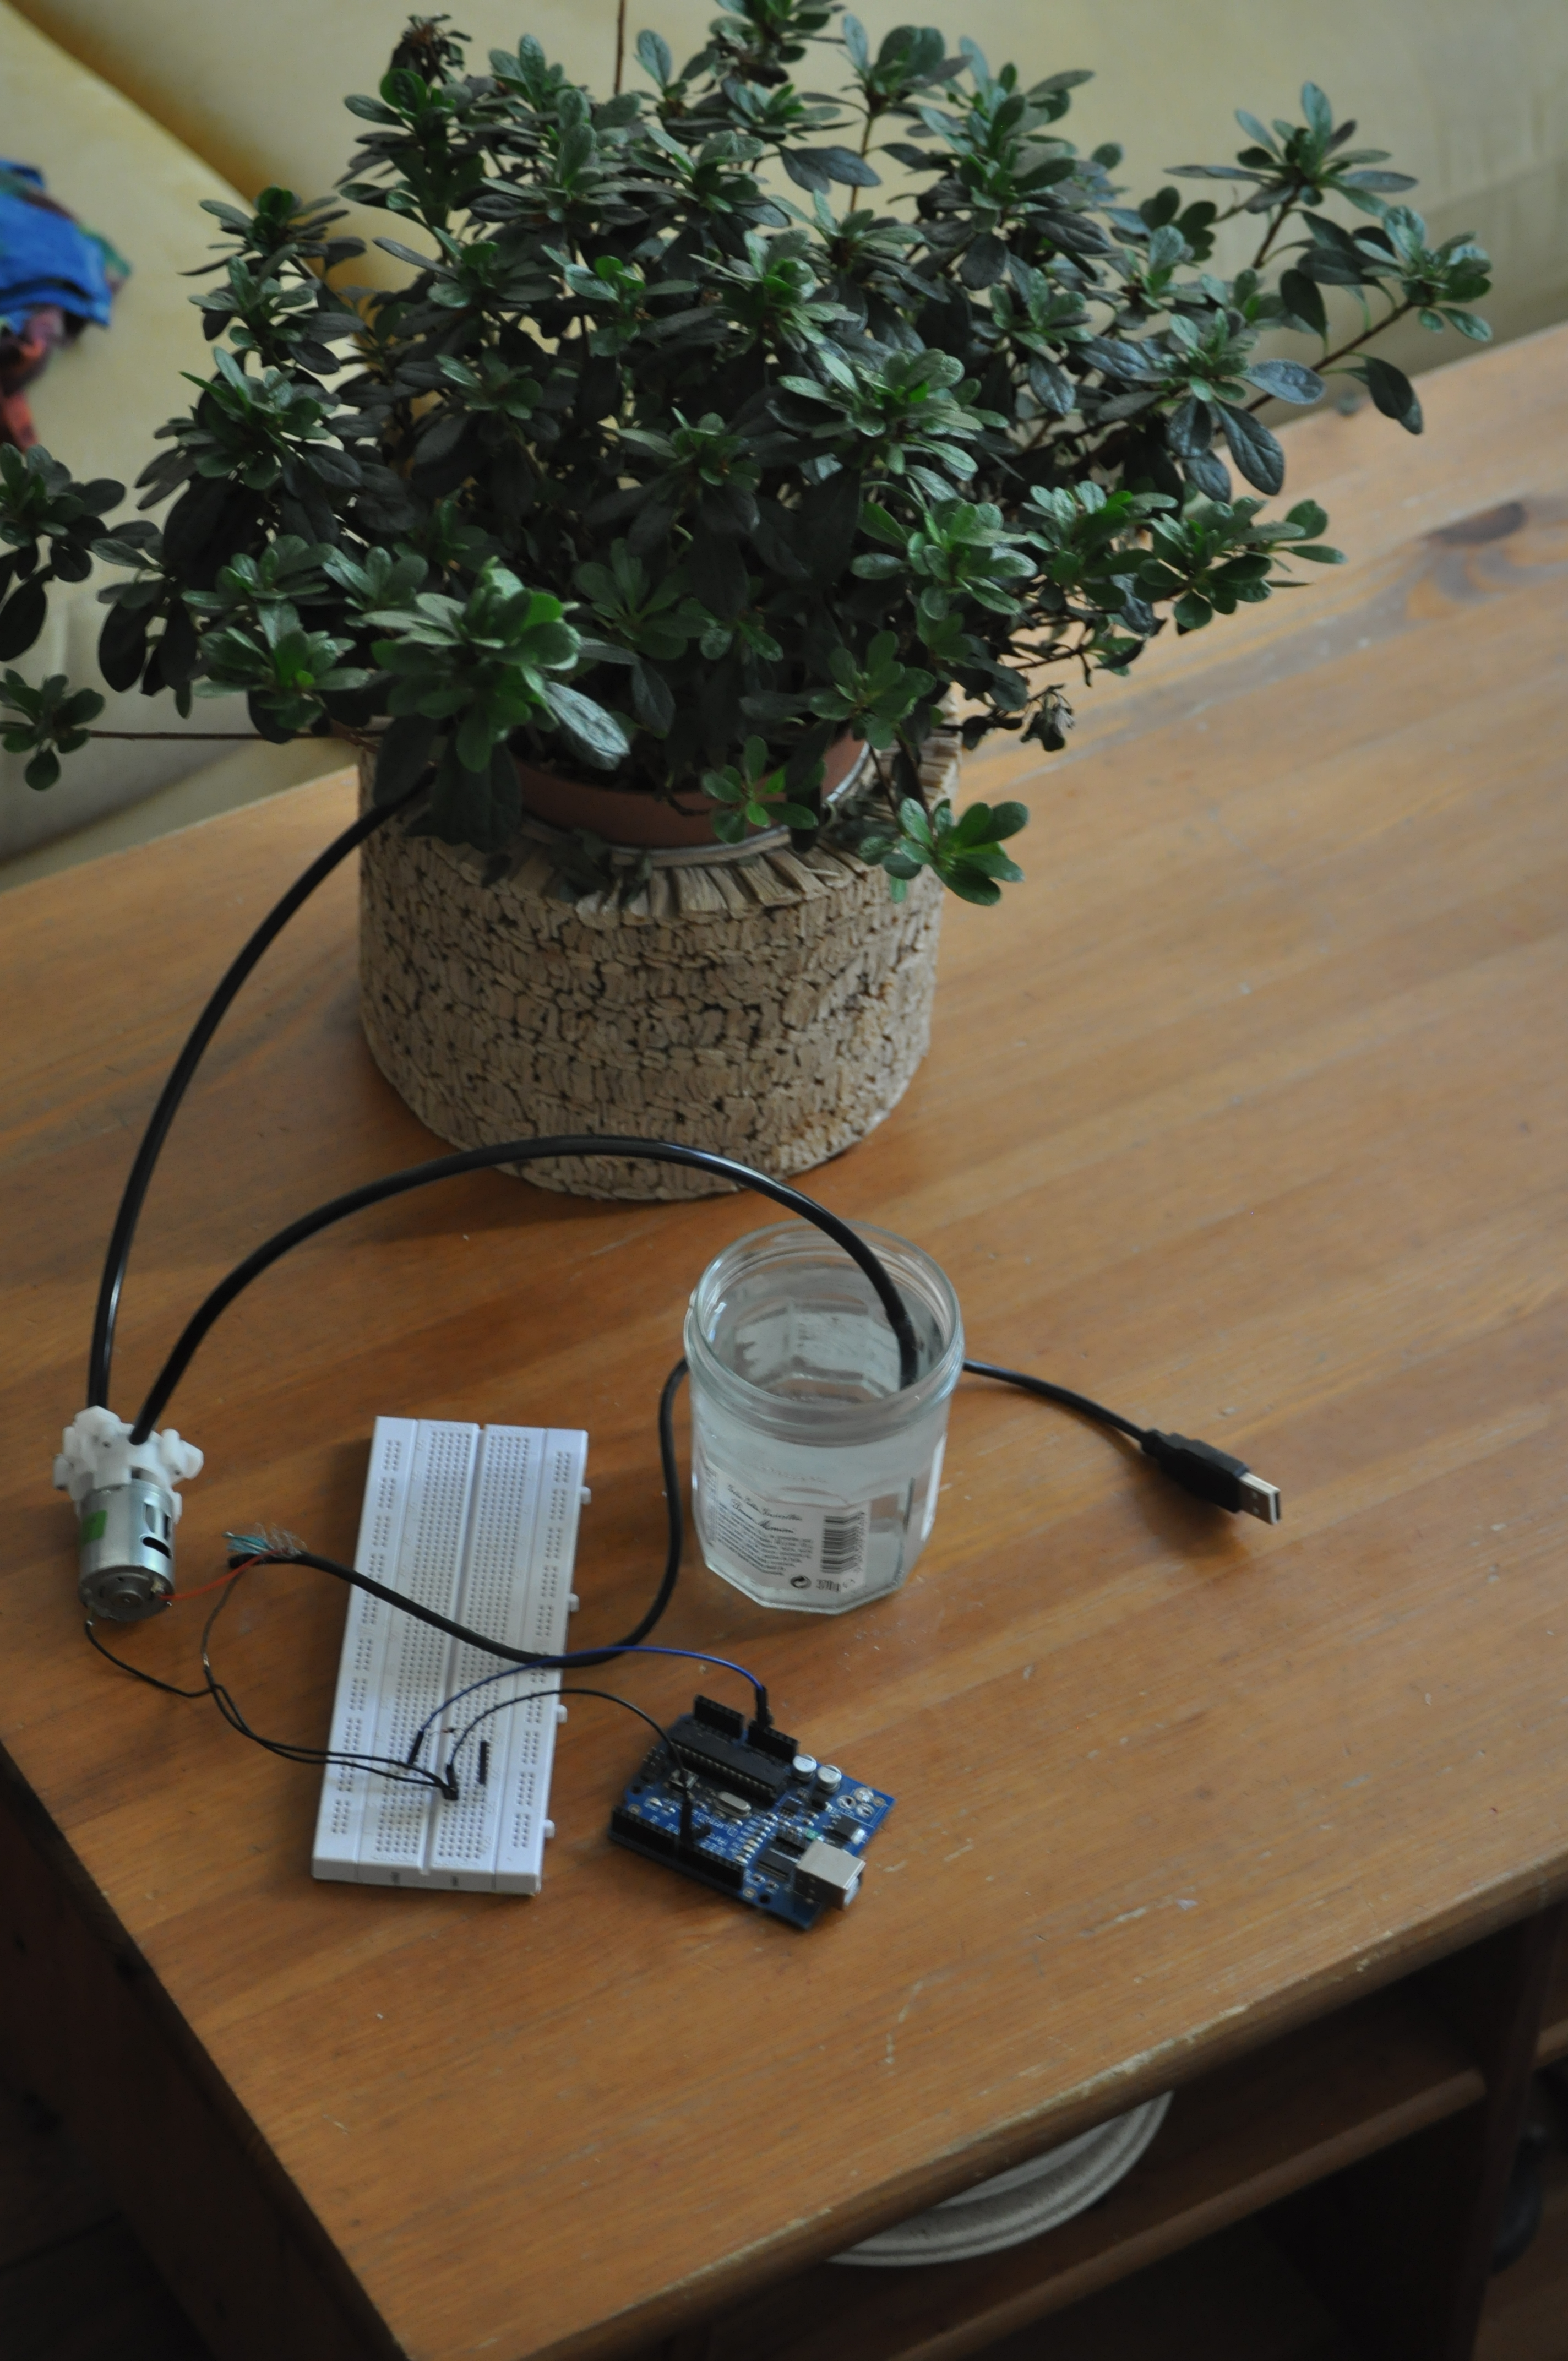
\includegraphics[width=\columnwidth]{final_plant}
    \caption{A plant connected to the automated watering system.}
    \label{fig:final_plant}
\end{figure}

%==============================================================================
\section{Automated Watering}
\label{sec:automated}

%------------------------------------------------------------------------------
\subsection{Measuring Moisture}

% related work

% conductivity

\begin{figure}
    \centering
    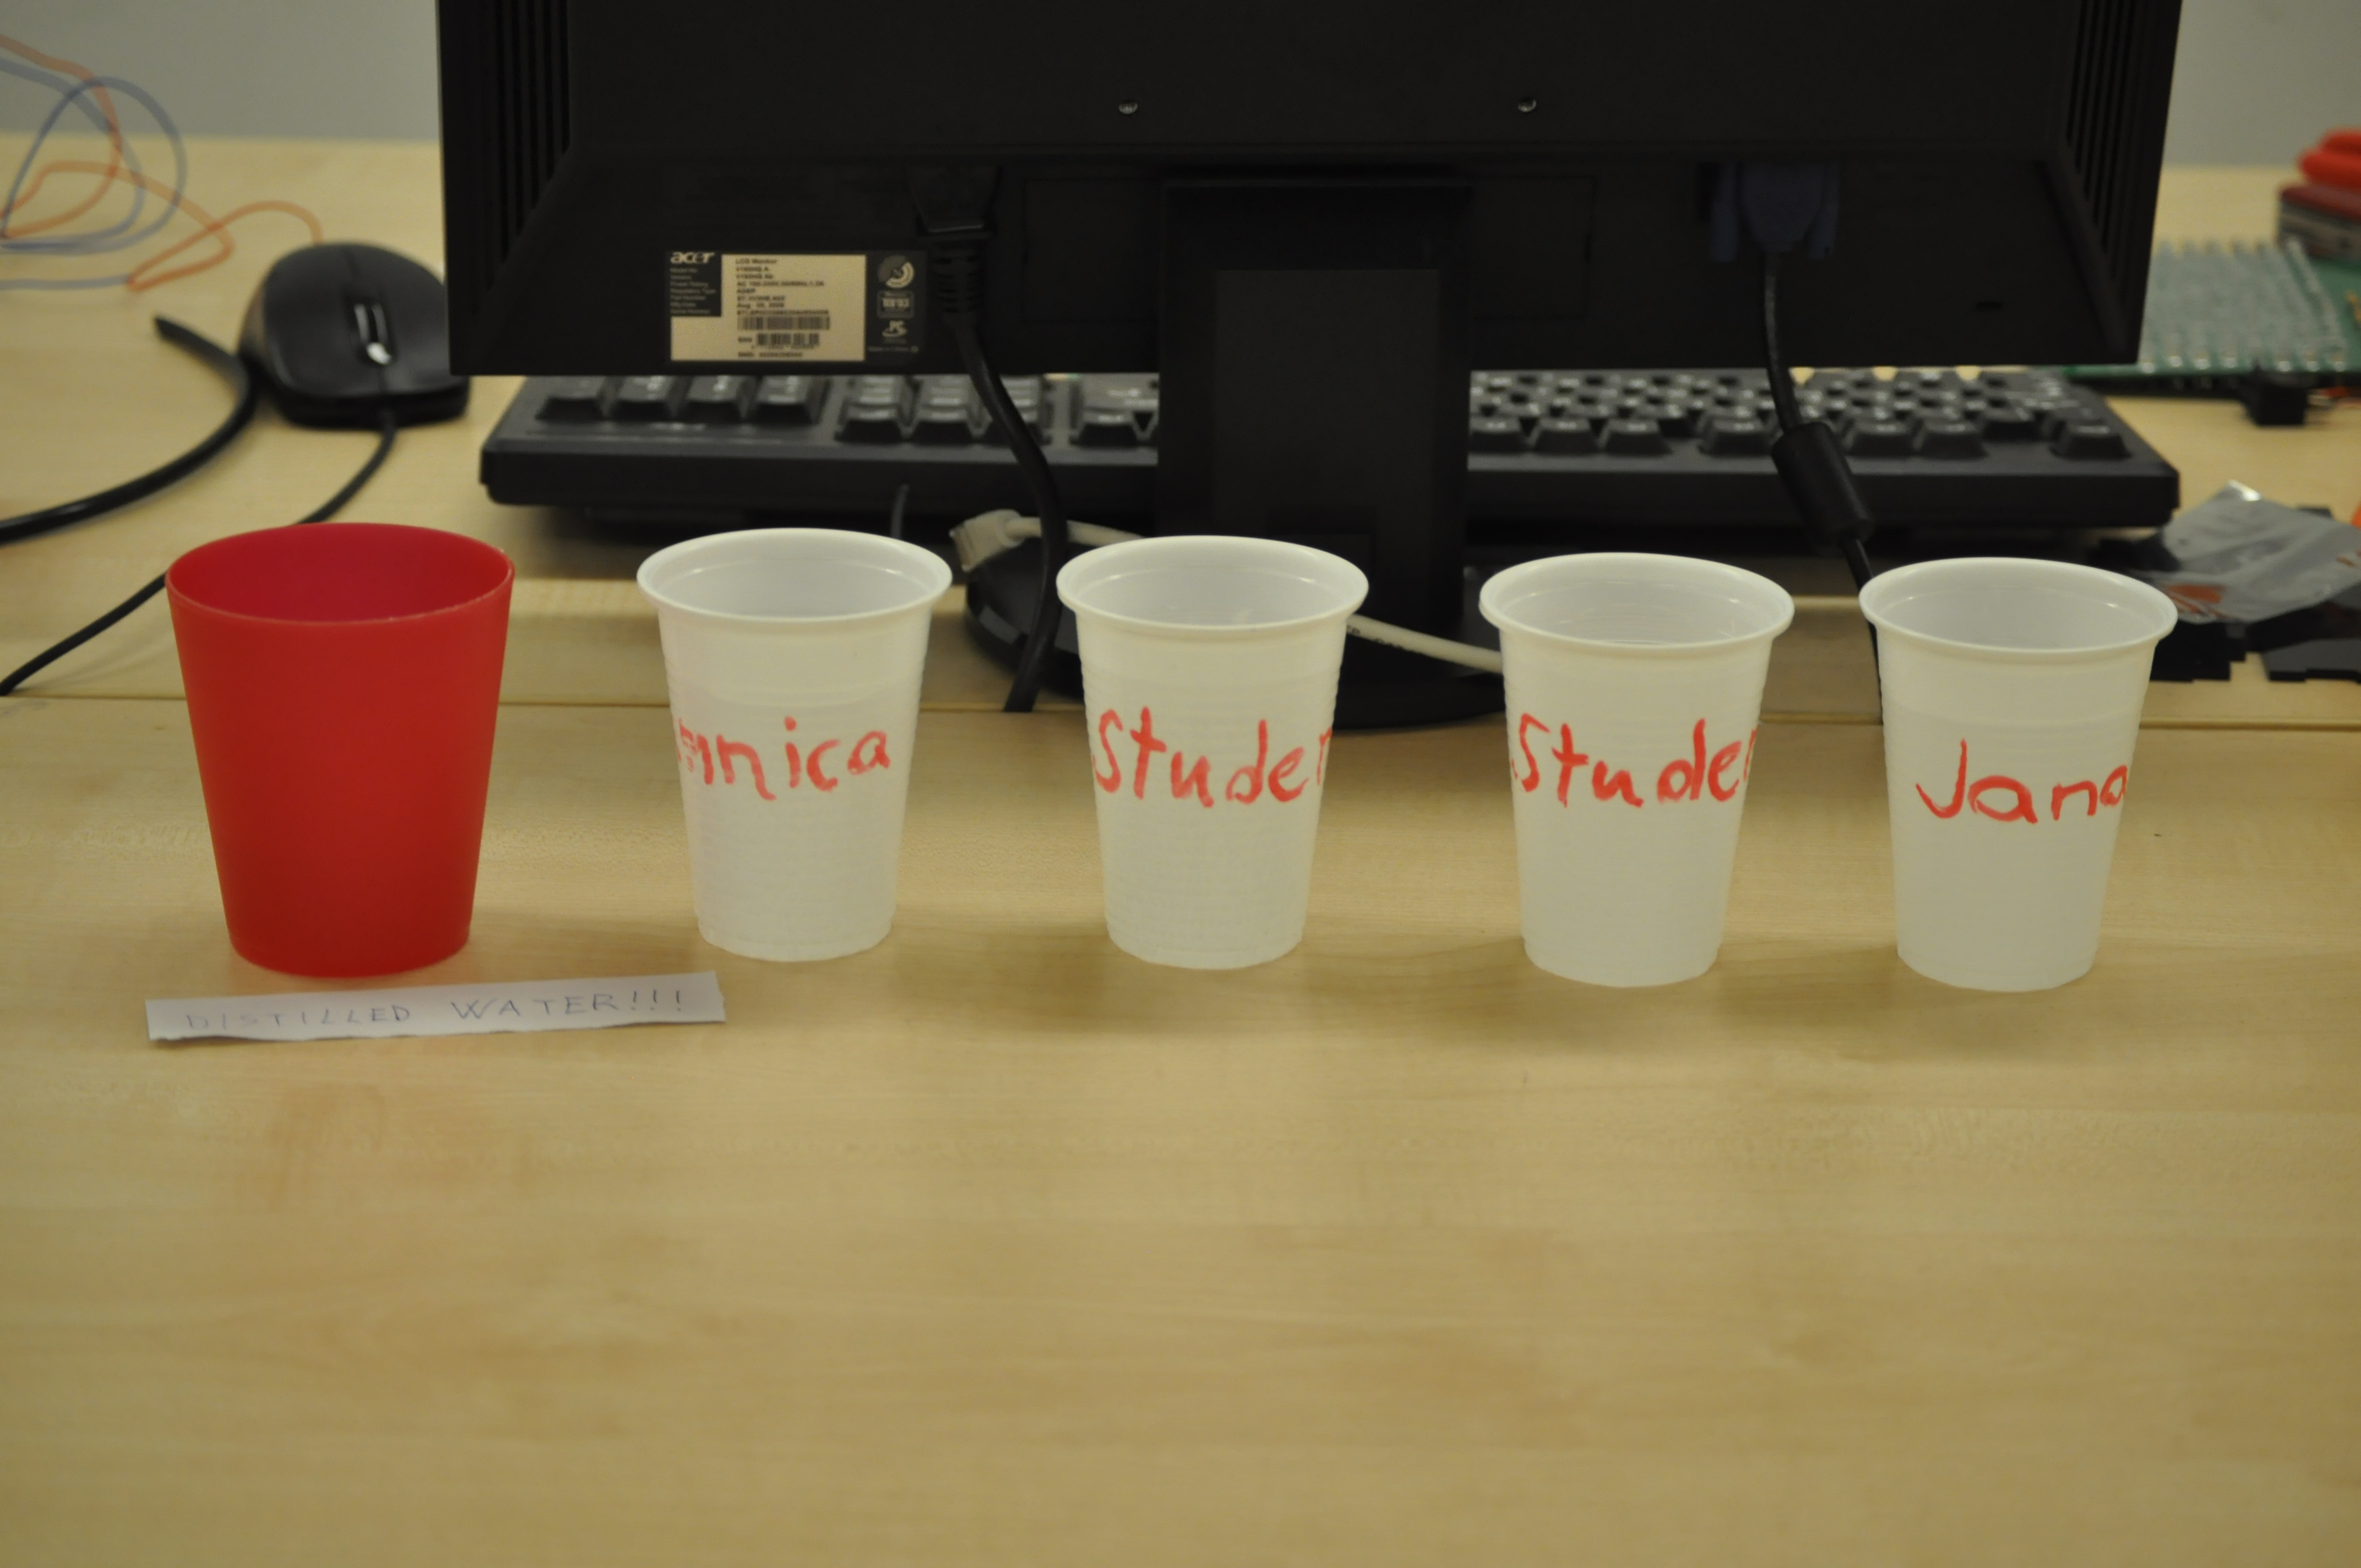
\includegraphics[width=\columnwidth]{water_testing}
    \caption{Different types of water show the same conductivity}
    \label{fig:water_testing}
\end{figure}

%------------------------------------------------------------------------------
\subsection{Watering System}

% arduino

% water pump

% circuit

\begin{figure}
    \centering
    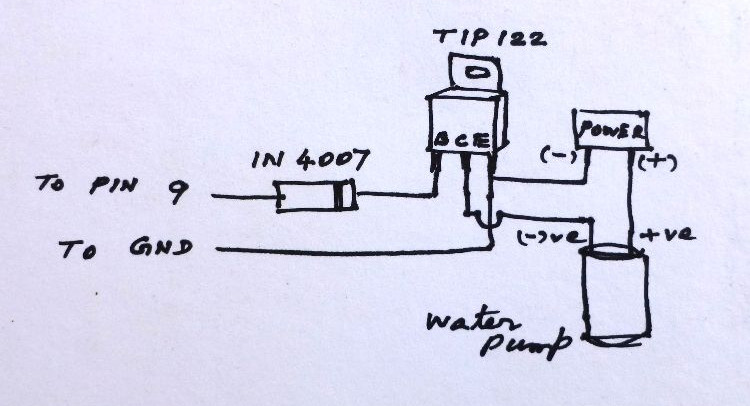
\includegraphics[width=\columnwidth]{circuit}
    \caption{The Watering electronical circuit.}
    \label{fig:circuit}
\end{figure}

%==============================================================================
\section{Data Collection and Hosting}
\label{sec:collection}

% intro

%------------------------------------------------------------------------------
\subsection{RF Communication}

% OOK

% interferences

%------------------------------------------------------------------------------
\subsection{Hosting}

% Web server


%==============================================================================
\section{Conclusion}
\label{sec:conclusion}

%==============================================================================
\section*{Acknowledgments}

% Summer School Organisation

% Maja for the water testing

%==============================================================================

\bibliographystyle{IEEEtran}
\begin{thebibliography}{10}
  \bibitem{toto}
    802.15.4-2011: IEEE Standard for Local and metropolitan area networks. Part
\end{thebibliography}

\end{document}
